% ==========================================================
% Term Project Report (continuation study)
% ENSO, the Indian Ocean Dipole and Sri Lankan rainfall
% ==========================================================

\documentclass{article}
\usepackage{spconf,amsmath,amssymb,graphicx}
\usepackage[hyphens]{url}
\usepackage[hidelinks,breaklinks]{hyperref}
\Urlmuskip=0mu plus 2mu\relax
\def\UrlBreaks{\do\/\do\-\do\.\do\_}

\usepackage{booktabs}
\usepackage{siunitx}
\usepackage{enumitem}
\usepackage{stfloats}

\def\x{{\mathbf x}}
\def\L{{\cal L}}

\title{Entangled Oceans: Separating ENSO and the Indian Ocean Dipole in Sri Lankan Rainfall}

\name{Your Name (Roll Number: XXXXX)} % TODO: fill in your name and roll number

\address{
Internship / Term Project Report\\
{[Course / Trimester]}\\[0.5em] % TODO
B.Sc. (Honours) Data Science and Artificial Intelligence\\
Indian Institute of Technology Guwahati, India\\
\texttt{your-email@op.iitg.ac.in} % TODO: fill in your email
}

\begin{document}
\ninept
\maketitle

% ==========================================================
\begin{abstract}
Sri Lankan rainfall is influenced by both the El Ni\~{n}o--Southern Oscillation (ENSO) and the
Indian Ocean Dipole (IOD), but the two modes often occur together, which complicates attribution.
Using the Oceanic Ni\~{n}o Index (ONI), a Dipole Mode Index (DMI) computed from OISST, and CHIRPS
rainfall for a south-western wet zone and a northern/eastern dry zone, this study asks how each mode
relates to rainfall over 1996--2025, how strongly the modes are related to each other, whether
either relates to North Indian Ocean cyclones, and what can be said for early 2027. All seven
positive-IOD years in the record (September--November DMI $\geq0.4^{\circ}$C) were El Ni\~{n}o years
(Fisher exact $p<0.0001$; $r=0.70$), so the IOD's separate effect cannot be identified from these
observations. October rainfall in the south-west rises with both indices ($r=+0.59$ for ONI, $+0.57$
for DMI; Benjamini--Hochberg $q=0.026$), but neither survives controlling for the other (partial
$r\approx+0.3$, $p\geq0.07$). February--April drying is an ENSO signal that persists after
controlling for the IOD (partial $r\approx-0.5$), and ONI alone gives the best cross-validated skill
in every season tested (0.13--0.38), with the DMI adding none. Cyclone counts show no ENSO or IOD
relationship; a weak association between a positive DMI and a larger Arabian Sea share of
post-monsoon storms ($\rho=+0.43$, $p=0.019$, 29 years) is reported as a hypothesis only. Scenario
outlooks for October--December 2026 and February--April 2027 tilt wetter and drier respectively,
but every 95\% prediction interval includes zero.
\end{abstract}

\begin{keywords}
Indian Ocean Dipole, El Ni\~{n}o, Sri Lanka, rainfall, tropical cyclones, seasonal outlook
\end{keywords}

% ==========================================================
\section{Introduction}
% ==========================================================

Sri Lanka's rainfall is organized around two monsoons and two inter-monsoon periods, and its
year-to-year variability has been linked to ENSO \cite{zubair2006,zubair2008,malmgren2003} and to the
IOD \cite{zubair2003,kajakokulan2025}. The IOD is a pattern of opposing sea-surface-temperature
anomalies between the western and south-eastern tropical Indian Ocean \cite{saji1999}, and it is well
known that dipole events can develop alongside El Ni\~{n}o, as in 1997--98 \cite{saji1999,webster1999}.
When two drivers co-occur, a correlation with either one is hard to attribute: the data may
simply record that both were present.

This matters now. As of the most recent data used here, the ONI had reached $+2.46^{\circ}$C
(August--October 2026), and the DMI computed in this study was $+0.64^{\circ}$C in September and
$+0.86^{\circ}$C in October 2026: a strong El Ni\~{n}o and a positive IOD developing together.
This study extends an earlier India/Sri Lanka ENSO analysis by asking what the IOD adds for
Sri Lanka specifically. Because the same CHIRPS record is used, the ENSO-only monthly results here
are not an independent replication of that earlier work.

Section~2 states the problem and objectives, Section~3 the data and methods, Section~4 the results,
Section~5 the discussion, and Section~6 the conclusions and future scope.

% ==========================================================
\section{Problem Statement and Objectives}
% ==========================================================

\textbf{Problem.} Does the IOD relate to Sri Lankan rainfall independently of ENSO, how closely are
the two modes coupled in 1996--2025, and can either mode support a defensible outlook for the
coming seasons?

\textbf{Objectives.}
\begin{itemize}[noitemsep]
    \item Compute a monthly DMI for 1996--2025 and identify IOD and ENSO events.
    \item Quantify the IOD--ENSO relationship and how often the two co-occur.
    \item Relate each index to Sri Lankan monthly and seasonal rainfall, separately and jointly,
    controlling for collinearity and multiple testing.
    \item Test for associations with North Indian Ocean cyclone frequency, location and intensity.
    \item Produce a cross-validated, scenario-based outlook for October--December 2026 and
    February--April 2027 with explicit uncertainty.
\end{itemize}

% ==========================================================
\section{Methodology}
% ==========================================================

\subsection{Data}
\textbf{ENSO.} The ONI was taken from NOAA CPC \cite{noaa_oni}. Years are classified by the
September--November (SON) mean ONI: El Ni\~{n}o $\geq+0.5^{\circ}$C, La Ni\~{n}a $\leq-0.5^{\circ}$C.

\textbf{IOD.} The DMI was computed from daily OISST v2.1 \cite{huang2021} retrieved through ERDDAP
\cite{erddap_oisst}, sub-sampled every $1^{\circ}$ for speed and area-averaged with $\cos(\text{lat})$
weights over the western box (50--70$^{\circ}$E, 10$^{\circ}$S--10$^{\circ}$N) and the south-eastern box
(90--110$^{\circ}$E, 10$^{\circ}$S--0$^{\circ}$), with anomalies relative to 1991--2020. A year is a
positive (negative) IOD year when its SON-mean DMI is $\geq+0.4$ ($\leq-0.4$)$^{\circ}$C; individual
events require $|\text{DMI}|\geq0.4^{\circ}$C for at least three consecutive months.

\textbf{Rainfall.} Monthly zone means of CHIRPS \cite{funk2015chirps} for two Sri Lankan zones,
south-west wet (79.6--80.6$^{\circ}$E, 6.0--7.3$^{\circ}$N) and north/east dry (80.4--81.9$^{\circ}$E,
5.9--9.9$^{\circ}$N), clipped to the island boundary. Anomalies are relative to each calendar month's
1996--2025 mean.

\textbf{Cyclones.} North Indian basin tracks from IBTrACS \cite{knapp2010,ibtracs_ni}, main tracks only.
A storm is a cyclonic storm if its maximum wind is $\geq34$~kt (IMD wind, falling back to JTWC where
missing). Post-monsoon storms form in October--December; a storm is ``near Sri Lanka'' if any track
point lies within 400~km of 7.8$^{\circ}$N, 80.7$^{\circ}$E.

\subsection{Mathematical formulation}
The dipole index is the difference of box-mean SST anomalies,
\begin{equation}
\text{DMI}_t=\bar{A}^{\mathrm{W}}_t-\bar{A}^{\mathrm{SE}}_t .
\end{equation}
Because monthly series are autocorrelated, correlations between full monthly series use an effective
sample size \cite{bretherton1999},
\begin{equation}
n_{\mathrm{eff}}=n\,\frac{1-r_{1x}r_{1y}}{1+r_{1x}r_{1y}},
\end{equation}
where $r_{1x},r_{1y}$ are lag-1 autocorrelations. To separate the two indices, partial correlations
hold the other index $z$ fixed,
\begin{equation}
r_{xy\cdot z}=\frac{r_{xy}-r_{xz}r_{yz}}{\sqrt{(1-r_{xz}^{2})(1-r_{yz}^{2})}},
\end{equation}
tested with $n-3$ degrees of freedom. Across $m$ simultaneous tests, Benjamini--Hochberg
\cite{benjamini1995} $q$-values $q_{(i)}=\min_{j\geq i}\{m\,p_{(j)}/j\}$ control the false-discovery
rate. Seasonal models $\hat{A}=\beta_0+\beta_1\text{ONI}+\beta_2\text{DMI}$ (or subsets) are scored by
leave-one-year-out cross-validation against a climatology baseline,
\begin{equation}
\text{SS}=1-\frac{\text{MSE}_{\text{model}}}{\text{MSE}_{\text{clim}}},
\end{equation}
so SS$>0$ means the model beats climatology out of sample. Predictions carry 95\% prediction intervals
$\hat{y}_0\pm t_{0.975}\,s\sqrt{1+\mathbf{x}_0^{\top}(X^{\top}X)^{-1}\mathbf{x}_0}$, with inputs
capped at the observed range to avoid extrapolation. Storm counts per year $N_y$ are modelled as
$\log\mathbb{E}[N_y]=\gamma_0+\gamma_1\text{ONI}_y+\gamma_2\text{DMI}_y$ (Poisson, robust errors).

% ==========================================================
\section{Experiments and Results}
% ==========================================================

\subsection{Setup}
All analysis ran in Python (\texttt{xarray}, \texttt{statsmodels}, \texttt{scipy}) in the notebook
listed in Section~7. The analysis period is 1996--2025 (30 years); 2026 values are used only to
describe the current event and to set outlook scenarios.

\subsection{The IOD and ENSO are tightly coupled}
Figure~\ref{fig:timeline} shows both indices. The DMI has standard deviation $0.47^{\circ}$C and
ranges from $-1.27$ to $+1.77^{\circ}$C; the record contains seven positive and eight negative IOD
events and nine El Ni\~{n}o events. Table~\ref{tab:cross} classifies the 30 years by their SON state.
All seven positive-IOD years (1997, 2002, 2006, 2015, 2018, 2019, 2023) were El Ni\~{n}o years, and
no La Ni\~{n}a or neutral year had a positive SON-mean DMI (Fisher exact $p<0.0001$). Two positive-IOD
events (2012, 2017) occurred in non-El Ni\~{n}o years but peaked outside September--November. The SON-mean
ONI--DMI correlation across years is $r=0.70$. By calendar month the coupling is seasonal
(Fig.~\ref{fig:bymonth}): significant from August to December and near zero in February--March.
For all months pooled, the lag correlation peaks near zero lag ($r\approx0.43$--$0.46$ at lags of
$-1$ to $0$ months, $n_{\mathrm{eff}}\approx53$), with no clear lead of one index over the other.

\begin{figure}[t]
    \centering
    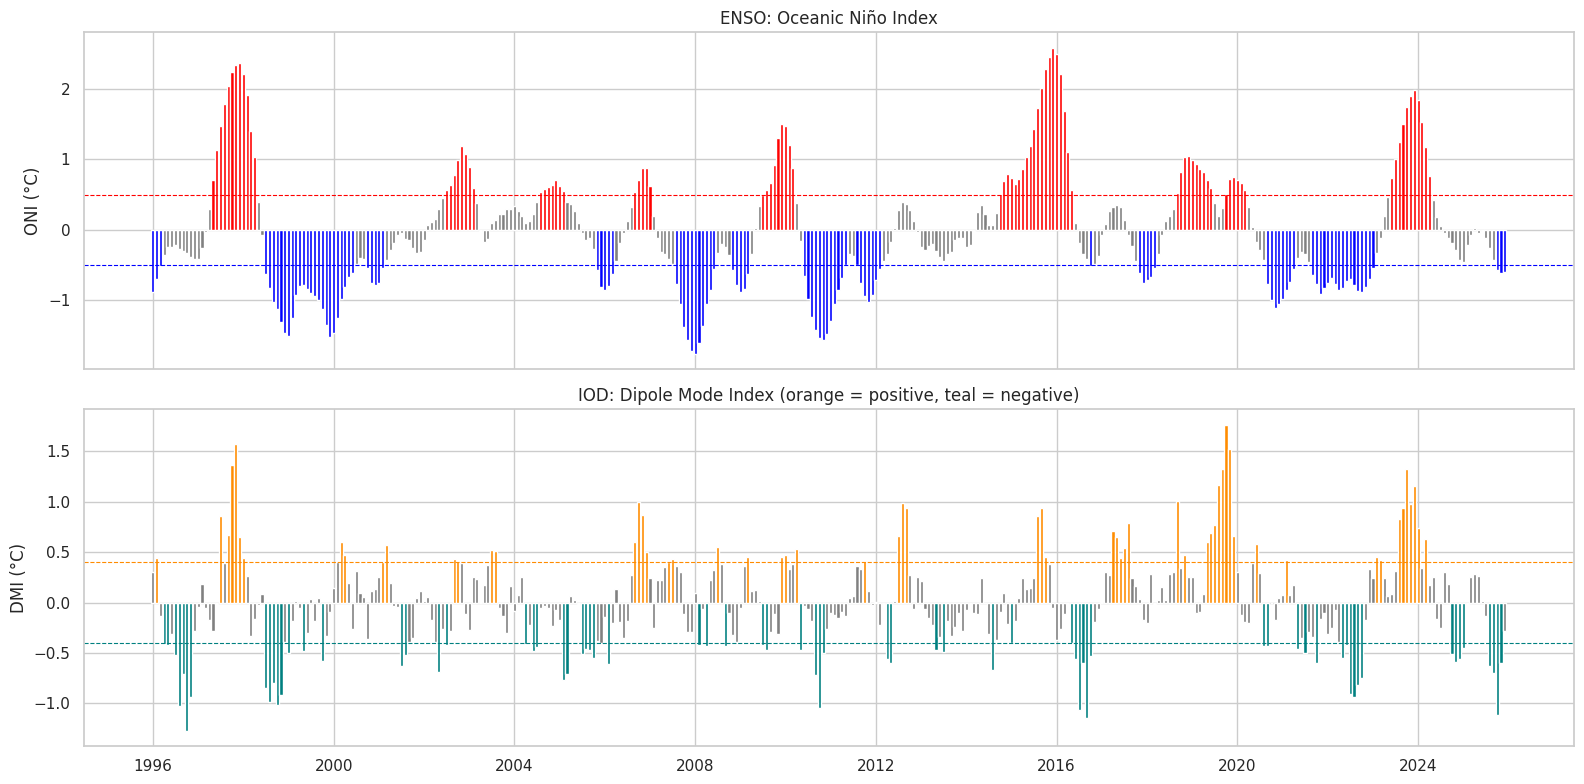
\includegraphics[width=\linewidth]{figures/oni_dmi_timeline.png}
    \caption{ONI (top) and DMI (bottom), 1996--2025. Colours mark El Ni\~{n}o/La Ni\~{n}a
    (ONI $\pm0.5$) and positive/negative IOD (DMI $\pm0.4$).}
    \label{fig:timeline}
\end{figure}

\begin{table}[t]
\centering
\footnotesize
\caption{Years classified by SON ENSO phase and IOD phase (30 years).}
\label{tab:cross}
\begin{tabular}{lcccc}
\toprule
ENSO phase & pIOD & Neutral IOD & nIOD & Total \\
\midrule
El Ni\~{n}o & 7 & 2 & 0 & 9 \\
La Ni\~{n}a & 0 & 6 & 4 & 10 \\
Neutral & 0 & 8 & 3 & 11 \\
\midrule
Total & 7 & 16 & 7 & 30 \\
\bottomrule
\end{tabular}
\end{table}

\begin{figure}[t]
    \centering
    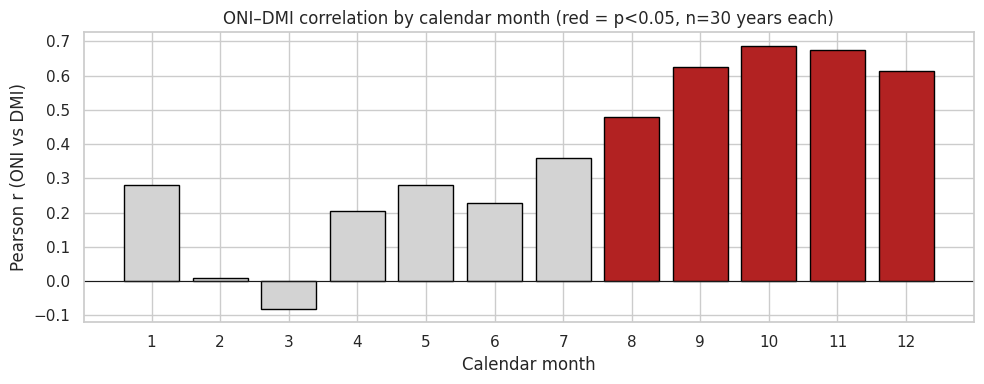
\includegraphics[width=\linewidth]{figures/oni_dmi_by_month.png}
    \caption{ONI--DMI correlation by calendar month (30 years each); red bars $p<0.05$.}
    \label{fig:bymonth}
\end{figure}

\subsection{Sri Lankan rainfall: monthly correlations}
Figure~\ref{fig:heat} gives the simple correlation of each index with rainfall anomalies for every
month and zone (48 tests). Table~\ref{tab:sel} lists the strongest, with partial correlations. The
October signal in the south-west is the strongest in the study ($r=+0.594$ for ONI, $+0.568$ for
DMI, $q=0.026$ for both), but when either index is held constant the other drops to
$r\approx+0.3$ and is not significant ($p=0.070$ and $0.153$). In the north/east the October DMI
association ($+0.505$) retains more than ONI after partialling ($+0.327$ vs $+0.118$), though neither
is significant. February--March drying with ONI is essentially unchanged by controlling for the DMI
(e.g.\ south-west February $-0.507\rightarrow-0.508$, $p=0.005$). None of the partial
correlations reaches $q<0.10$ (smallest $q=0.158$), so partialled results are suggestive rather than
confirmed after false-discovery control. The positive north/east May ONI correlation ($+0.450$)
is unexplained and should be treated with caution.

\begin{figure*}[t]
    \centering
    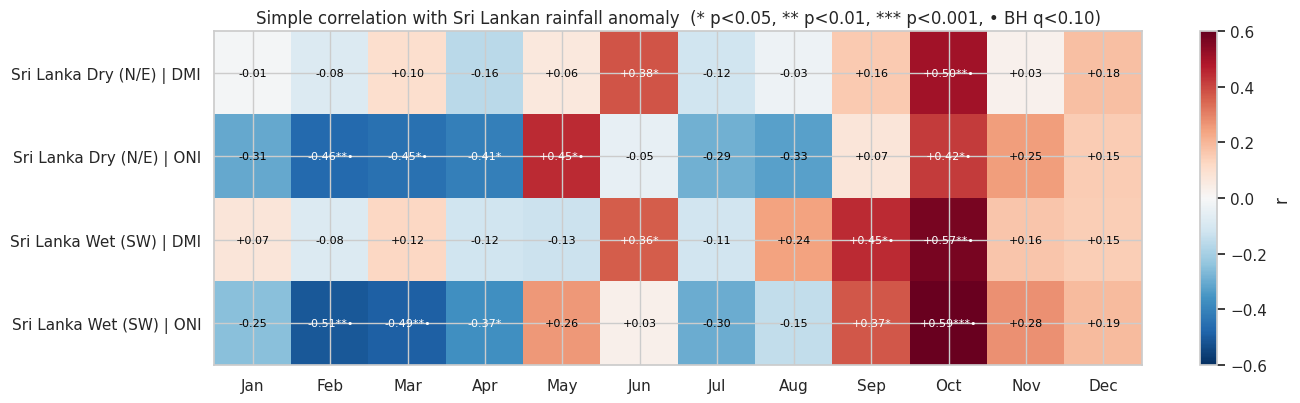
\includegraphics[width=0.92\textwidth]{figures/sl_heatmap_simple.png}
    \caption{Correlation of ONI and DMI with Sri Lankan rainfall anomalies by month and zone
    (* $p<0.05$, ** $p<0.01$, *** $p<0.001$; $\bullet$ marks Benjamini--Hochberg $q<0.10$).}
    \label{fig:heat}
\end{figure*}

\begin{table}[t]
\centering
\footnotesize
\setlength{\tabcolsep}{3pt}
\caption{Selected monthly correlations: simple $r$ (BH $q$) and partial $r$ ($p$) with the other
index held constant. SW = south-west wet, NE = north/east dry.}
\label{tab:sel}
\begin{tabular}{llcccc}
\toprule
Zone & Month & Index & $r$ ($q$) & Partial $r$ ($p$) \\
\midrule
SW & Oct & ONI & $+0.594$ (0.026) & $+0.341$ (0.070) \\
SW & Oct & DMI & $+0.568$ (0.026) & $+0.272$ (0.153) \\
NE & Oct & DMI & $+0.505$ (0.053) & $+0.327$ (0.084) \\
NE & Oct & ONI & $+0.421$ (0.098) & $+0.118$ (0.542) \\
SW & Feb & ONI & $-0.507$ (0.053) & $-0.508$ (0.005) \\
SW & Mar & ONI & $-0.490$ (0.058) & $-0.485$ (0.008) \\
NE & Feb & ONI & $-0.465$ (0.072) & $-0.466$ (0.011) \\
NE & Mar & ONI & $-0.446$ (0.072) & $-0.442$ (0.016) \\
\bottomrule
\end{tabular}
\end{table}

\subsection{Seasonal models and analog years}
Table~\ref{tab:skill} compares models for October--December (OND) and February--April (FMA) mean
rainfall. ONI alone has the best cross-validated skill in every case; adding the DMI lowers it.
In the OND models the two indices are strongly collinear ($r=0.70$) and, together, neither is
significant (south-west: ONI $p=0.086$, DMI $p=0.454$); in FMA the indices are nearly uncorrelated
($r=0.05$) and the DMI coefficient is null ($p=0.947$).

\begin{table}[t]
\centering
\footnotesize
\caption{Leave-one-year-out MSE skill score versus climatology (SW = south-west wet, NE = north/east
dry) and the ONI--DMI correlation within each window.}
\label{tab:skill}
\begin{tabular}{llcccc}
\toprule
Zone & Window & ONI & DMI & ONI+DMI & $r_{\text{ONI,DMI}}$ \\
\midrule
SW & OND & 0.220 & 0.143 & 0.201 & 0.70 \\
SW & FMA & 0.323 & $-0.069$ & 0.272 & 0.05 \\
NE & OND & 0.128 & 0.087 & 0.106 & 0.70 \\
NE & FMA & 0.382 & $-0.037$ & 0.369 & 0.05 \\
\bottomrule
\end{tabular}
\end{table}

Because regression cannot separate collinear drivers, Table~\ref{tab:analog} shows what the present
combination (El Ni\~{n}o with a positive IOD) produced in the past. For FMA the preceding SON state
is used. The seven analog years differ from all other years (Mann--Whitney $p=0.007$--$0.029$), but
only two El Ni\~{n}o years lacked a positive IOD (2004 and 2009), so the comparison that would isolate
the IOD has almost no power ($p=0.22$--$1.0$).

\begin{table}[t]
\centering
\footnotesize
\setlength{\tabcolsep}{2.5pt}
\caption{Mean rainfall anomaly (mm/day) by SON category. $p$: Mann--Whitney, El Ni\~{n}o+pIOD
($n=7$) versus all other years.}
\label{tab:analog}
\begin{tabular}{llccccc}
\toprule
Zone & Window & EN+pIOD & EN, no pIOD & La Ni\~{n}a & Neutral & $p$ \\
\midrule
SW & OND & $+2.79$ & $+0.45$ & $-0.88$ & $-1.06$ & 0.007 \\
SW & FMA & $-1.85$ & $+0.08$ & $+1.84$ & $-0.21$ & 0.018 \\
NE & OND & $+1.32$ & $+1.37$ & $-0.30$ & $-0.82$ & 0.029 \\
NE & FMA & $-1.33$ & $-0.26$ & $+1.13$ & $+0.03$ & 0.013 \\
\bottomrule
\end{tabular}
\end{table}

\subsection{North Indian Ocean cyclones}
There are 170 cyclonic storms in 1996--2025 (5.67 per year), of which 94 formed in October--December
(3.13 per year) and 0.80 per year passed within 400~km of Sri Lanka. Storm counts show no
relationship with either index (Table~\ref{tab:cyc}); mean OND counts are 3.22, 2.80 and 3.36 in
El Ni\~{n}o, La Ni\~{n}a and neutral years, and 3.43, 3.00 and 3.06 in positive, negative and neutral
IOD years. The only pattern is in genesis location: storm-level genesis longitude falls with the DMI
($\rho=-0.32$, $p=0.002$, 94 storms), but storms in one year share one DMI value. At year level
($n=29$) the association is weaker ($\rho=-0.37$, $p=0.049$), and the Arabian Sea share of
post-monsoon storms rises with the DMI ($\rho=+0.43$, $p=0.019$). About 22 tests were run in
this section, so one nominal $p<0.05$ is expected by chance alone.

\begin{table}[t]
\centering
\footnotesize
\setlength{\tabcolsep}{3pt}
\caption{Cyclone tests: Poisson coefficient $\gamma$ ($n=30$ years) or Spearman $\rho$ ($n=29$
years), with $p$ in parentheses.}
\label{tab:cyc}
\begin{tabular}{lccc}
\toprule
Outcome (per year) & Test & ONI & DMI \\
\midrule
Post-monsoon storm count & $\gamma$ & $-0.078$ (0.36) & $+0.197$ (0.26) \\
Storms within 400 km & $\gamma$ & $-0.168$ (0.42) & $+0.180$ (0.50) \\
Mean genesis longitude & $\rho$ & $-0.23$ (0.23) & $-0.37$ (0.049) \\
Arabian Sea share & $\rho$ & $+0.36$ (0.057) & $+0.43$ (0.019) \\
Peak wind & $\rho$ & $-0.03$ (0.89) & $+0.23$ (0.23) \\
\bottomrule
\end{tabular}
\end{table}

\subsection{Scenario outlook}
Table~\ref{tab:out} applies the ONI-only model, the best cross-validated model in every window, to
scenario ONI values. These are scenarios, not forecasts. Inputs above the observed maximum of the
window mean ($\approx2.4$ for OND, $\approx1.7$ for FMA) are capped at it (marked *).

\begin{table}[t]
\centering
\footnotesize
\setlength{\tabcolsep}{3pt}
\caption{ONI-only outlook: mean anomaly (mm/day) with 95\% prediction interval. Skill is from
Table~\ref{tab:skill}.}
\label{tab:out}
\begin{tabular}{llcl}
\toprule
Window & Zone (skill) & ONI & Anomaly [95\% PI] \\
\midrule
OND 2026 & SW (0.22) & 2.0 & $+3.04$ [$-2.87$, $+8.95$] \\
 & & 2.5* & $+3.70$ [$-2.36$, $+9.76$] \\
 & NE (0.13) & 2.0 & $+1.70$ [$-2.98$, $+6.37$] \\
 & & 2.5* & $+2.06$ [$-2.73$, $+6.85$] \\
FMA 2027 & SW (0.32) & 1.0 & $-2.02$ [$-6.07$, $+2.03$] \\
 & & 1.5 & $-3.00$ [$-7.20$, $+1.19$] \\
 & & 2.0* & $-3.34$ [$-7.59$, $+0.91$] \\
 & NE (0.38) & 1.0 & $-1.40$ [$-4.00$, $+1.19$] \\
 & & 1.5 & $-2.09$ [$-4.77$, $+0.60$] \\
 & & 2.0* & $-2.32$ [$-5.04$, $+0.40$] \\
\bottomrule
\end{tabular}
\end{table}

% ==========================================================
\section{Discussion}
% ==========================================================

\textbf{Entanglement limits attribution.} In this sample no year had a positive SON-mean DMI without
El Ni\~{n}o (the 2012 and 2017 events lay mostly outside SON), and the SON indices correlate at 0.70. The October association with the DMI therefore
cannot be separated from ENSO, and the October result should be described as belonging to
El Ni\~{n}o/positive-IOD years rather than to either mode. This is consistent with earlier work
reporting IOD links to Sri Lankan Maha-season rainfall \cite{zubair2003,zubair2008,kajakokulan2025}
and ENSO links to northeast-monsoon rainfall \cite{zubair2006}: both can be present in the data
without the record being able to apportion them.

\textbf{February--April is an ENSO signal.} The negative ONI correlation in February--April is
unchanged by controlling for the DMI and the indices are almost uncorrelated in this window. This
agrees with published findings of a negative Ni\~{n}o~3.4 relationship with January--April
rainfall over southern India and Sri Lanka \cite{vialard2011,lin2026}, which also found it
persisted after controlling for an Indian Ocean temperature-gradient index. Honest caveats remain:
no partial test passes $q<0.10$, and the FMA window was chosen after the same data had been seen in
the earlier study, so its cross-validated skill is optimistic.

\textbf{The DMI adds no out-of-sample skill.} ONI alone matched or beat every combined model
(Table~\ref{tab:skill}). This is evidence of no demonstrated added value in 30 years, not
evidence that the IOD has no influence; the sample simply lacks El Ni\~{n}o years without a
positive IOD (two) and positive-IOD (SON) years without El Ni\~{n}o (none). The analog table shows the
same limit: the six-to-seven analog years differ from other years, but nothing isolates the IOD.

\textbf{Cyclones.} Earlier studies describe La Ni\~{n}a and negative-IOD conditions as more
favourable for post-monsoon Bay of Bengal cyclone activity \cite{girishkumar2012,mahala2015}. Our
basin-wide counts do not show this contrast (La Ni\~{n}a 2.80 versus El Ni\~{n}o 3.22 storms per
year; negative IOD 3.00 versus positive IOD 3.43), though none of these differences is
distinguishable from zero. Differences in domain (whole North Indian Ocean versus the Bay of Bengal),
storm definition, wind threshold and period could contribute, and 30 years has little power to
detect count differences of this size. The genesis-location association with the DMI is a
hypothesis worth testing on a longer record, not a finding.

\textbf{Outlook.} Every 95\% prediction interval includes zero, so the models shift the odds toward a
wetter late 2026 and a drier February--April 2027 without fixing an outcome. The tilt for
February--April has the better support (skill 0.32--0.38); the October--December skill is lower
(0.13--0.22). The ENSO inputs are scenarios, and nothing here supports statements beyond mid-2027.

\textbf{Limitations.} The DMI was computed from a $1^{\circ}$ sub-sample of OISST with a 1991--2020
baseline and was not cross-checked against an independent DMI product in this version. The zones are
approximate bounding boxes, the sample is 30 years, and the ENSO-only monthly results reuse the CHIRPS
record of the earlier study. The cyclone analysis uses one wind threshold, a 400~km radius, and
14 post-monsoon storms carrying an unassigned sub-basin code.

% ==========================================================
\section{Conclusion and Future Work}
% ==========================================================

In 1996--2025 the IOD and ENSO were tightly coupled: every positive-IOD year was an El Ni\~{n}o year.
As a result, Sri Lanka's October rainfall increase cannot be assigned to either mode, whereas the
February--April decrease is an ENSO signal that survives controlling for the IOD. ONI alone gave the
best cross-validated skill, cyclone frequency showed no ENSO or IOD relationship, and scenario
outlooks for late 2026 and February--April 2027 tilt wetter and drier but with prediction intervals
that include zero.

\textbf{Future scope.}
\begin{itemize}[noitemsep]
    \item Cross-check the DMI against NOAA PSL/JAMSTEC products and test detrended variants.
    \item Extend the record (longer gauge or satellite data) to obtain more independent IOD events,
    especially El Ni\~{n}o without a positive IOD and the reverse.
    \item Test lagged predictors (SON ONI/DMI for February--April rainfall) and station-level data.
    \item Compare the statistical outlook with dynamical seasonal forecasts and calibrate.
    \item Repeat the cyclone analysis for the Bay of Bengal alone using accumulated cyclone energy
    and sub-basin definitions, with a sensitivity test on the wind threshold.
    \item Use short-range AI forecasts (e.g.\ WeatherNext) only for operational now-casting, kept
    separate from seasonal claims.
\end{itemize}

% ==========================================================
\section{Artifacts and Demonstrations}
% ==========================================================

\begin{itemize}[noitemsep]
    \item \textbf{Code Repository:} \url{https://github.com/username/project-name} % TODO: add your repo link
    \item \textbf{Notebook:} IOD\_ENSO\_SriLanka\_Continuation.ipynb % TODO: update as needed
\end{itemize}

\textbf{Note on AI assistance:} AI-assisted tools were used during code development and drafting, as
permitted by the course; the author is responsible for all analysis choices, results and
interpretation. % TODO: confirm this wording against your course policy

% ==========================================================
\vfill\pagebreak
{\fontsize{8}{9}\selectfont
\bibliographystyle{IEEEbib}
\bibliography{refs}
}

\end{document}
